
\chapter{Die STG-Sprache}\label{chap:stg}

Die \gls{stg}-Sprache ist eine kleine funktionale Programmiersprache, die eng mit der Semantik der \gls{stg}-Maschine verknüpft ist.
Zudem dient sie als kleiner Sprachkern für Haskell und wird dort im Übersetzungs- und Ausführungsprozess verwendet.

Im Vergleich zu anderen Maschinensprachen fällt auf, dass die \gls{stg}-Sprache eine funktionale Programmiersprache ist.
Anstelle der Beschreibung einzelner Anweisungen oder Instruktionen, die den Zustand der Maschine ändern, werden deklarativ Funktionen beschrieben, deren Zusammenspiel einen Graphen bildet.
Da die Reduktion dieses Graphen der Ausführung der \gls{stg}-Maschine entspricht, gibt es einige Unterschiede zu funktionalen Kern- oder Hochsprachen.
Anstelle viele, einfache Abstraktionen zu schaffen, ist eine genaue Kontrolle über das Verhalten der zugrundeliegenden Maschine gewünscht.

Sowohl die Nähe zur Maschinensemantik als auch die Kontrolle der selben wird bei Betrachtung der verschiedenen Sprachkonstrukte deutlich, die im Folgenden vorgestellt werden.

\begin{figure}
  \centering
  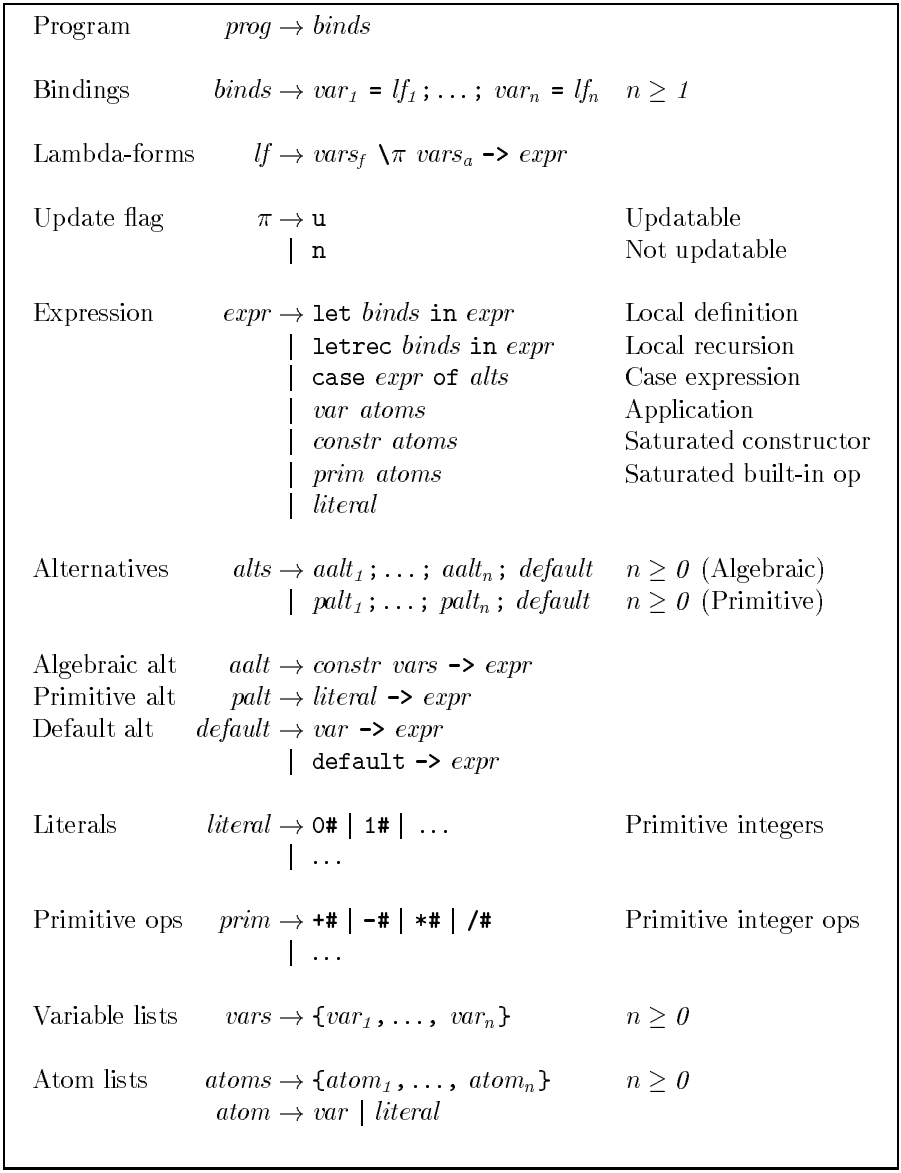
\includegraphics[width=\textwidth]{grammar}
  \caption[Grammatik der STG-Sprache]{Grammatik der STG-Sprache aus \cite{Jones_StockHardwareSTG}}\label{fig:grammar}
\end{figure}

\section{Lambdaformen}

Lambdaformen entsprechen den klassischen Lambdaausdrücken, wie sie aus nahezu allen funktionalen Sprachen bekannt sind.
Zusätzlich zu der Liste an Variablen, an welche die Argumente der anonymen Funktion gebunden werden, und dem Rumpf der Funktion existieren einige Besonderheiten.

Eine zusätzliche Liste an Variablen bei der Definition einer Lambdaform beschreibt die freien Variablen, die beim Erstellen einer Closure gespeichert werden müssen.
Freie Variablen sind Variablen, die in einem Ausdruck verwendet werden, jedoch nicht innerhalb dieses Ausdrucks definiert werden.
Sie entstehen also durch eine umschließende Definition, und müssen als Kontext der Funktion gespeichert werden.
Da dies Speicherplatz benötigt und somit die Ausführung der \gls{stg}-Maschine beeinflusst, werden die freien Variablen explizit angegeben.

Weiterhin fällt auf, dass eine \textit{Update Flag} als Teil der Lambdaform angegeben wird.
Ist diese Flagge auf \texttt{u} gesetzt, wird die Closure im Speicher nach der Auswertung durch den Ergebniswert ersetzt.
Somit wird eine erneute Auswertung unterbunden, die Performance erhöht und keine zusätzliche Berechnungen durchgeführt.
In anderen Fällen ist diese Ersetzung nicht erwünscht.
Wird ein Wert beispielsweise nur einmal berechnet, muss keine Ersetzung stattfinden und der dafür benötigte Aufwand kann eingespart werden.
Ähnlich ist es, wenn die Lambdaform eine Funktion beschreibt, oder der Ausdruck im Rumpf bereits in der \gls{whnf} ist (siehe~\cite[Chap. 4.2]{Jones_StockHardwareSTG}).


\section{Let-Bindungen}

Bindungsausdrücke binden (potentiell mehrere) Lambdaformen an Bezeichner.
Hierbei wird zwischen Bindungsausdrücken mit dem Schlüsselwort \texttt{let} und rekursiven Bindungsausdrücken mit dem Schlüsselwort \texttt{letrec} unterschieden.
Bei Letzterem dürfen die Definitionen des Ausdrucks gegenseitige Querbezüge besitzen.
Bei der ersten Variante ist dies nicht erlaubt.

Als Besonderheit fällt auf, dass lediglich Lambdaformen gebunden werden können.
Dies reflektiert die lazy Evaluation, da so nicht ein Ausdruck selbst oder dessen Wert gebunden wird.

Hinsichtlich der Maschinensemantik beschreiben Bindungsausdrücke immer Speicherallokation.
Für jede gebundene Lambdaform wird eine Closure auf dem Heap angelegt und die Referenz auf diese für die gebundene Variable verwendet.


\section{Anwendungen}

Die \gls{stg}-Maschine kennt Anwendungen von Funktionen, Konstruktoren und primitiven Operationen.
Im Vergleich zu Haskell gilt hier die Einschränkungen, dass die Anwendungen von Konstruktoren und primitiven Operationen immer alle Argumente angegeben sein müssen.
Eine $\eta$-Reduktion, wie sie in Haskell üblich und idiomatisch ist, wird hier nicht durchgeführt.
So ist sichergestellt, dass immer genügend Argumente auf dem Stack liegen, wenn diese Konstrukte ausgewertet werden, wodurch das Erreichen der \gls{whnf} bei der Auswertung von Konstruktoranwendungen und Aufrufe von primitiven Operationen sichergestellt wird.

Als Einschränkungen gilt für diese Ausdrücke, dass die übergebenen Argumente bei einer Anwendung immer atomar sein müssen; lediglich primitive Konstanten und Variablen sind erlaubt.
Dies reduziert die Komplexität der Maschine und erzwingt, dass komplexe Argumente, die ausgewertet werden müssten, explizit als Closure auf dem Heap abgelegt werden, bevor diese als Argument übergeben werden.

Soll eine einzelne Variable als Ausdruck verwendet werden, so muss die Variable als Funktion auf eine leere Parameterliste angewandt werden.
Bei der Auswertung dieses Ausdrucks wird dann zum Rumpf der Closure gesprungen, die an diese Variable gebunden wird.
Diese etwas umständliche Einschränkung bildet syntaktisch direkt das Ausführungsmodell der \gls{stg}-Maschine ab, in der jeder Ausdruck verzögert ausgewertet wird.

\section{Fallunterscheidungen}

Fallunterscheidungen bestehen aus einem untersuchten Ausdruck und einer Reihe an Fällen, die jeweils ein Muster definieren.
Der erste Fall, dessen Muster zu dem untersuchten Ausdruck passt, wird dabei als Ergebnis der Fallunterscheidung ausgewählt.
Ist kein passendes Muster gegeben, so tritt ein Laufzeitfehler auf.

Fallunterscheidungen sind einstufig; sie können nur anhand des äußersten Konstruktors oder einer primitiven Konstante getroffen werden.
Zudem darf ein Standardfall definiert werden, der immer akzeptiert und optional den gesamten Ausdruck an einen Namen bindet.
In der Praxis stellt diese Einschränkung kein Problem dar, da mehrstufige Fallunterscheidungen in einstufige übersetzt werden können~\cite{Wadler_PatternMatching}.

Die Besonderheit in der Semantik von Fallunterscheidungen ist, dass der untersuchte Ausdruck ausgewertet wird.
Somit bieten Fallunterscheidungen die einzige Möglichkeit in der \gls{stg}, die Auswertung eines Ausdrucks zu erzwingen.
Durch die Auswertung des untersuchten Ausdrucks in \gls{whnf} wird sichergestellt, dass der korrekte Fall ausgewählt wird, da nach der Auswertung der passende Konstruktor in ausgewerteter Form vorliegt.
Gleichzeitig wird dabei sichergestellt, dass nicht zu viel ausgewertet wird und die Laziness erhalten bleibt.


\section{Primitive Werte und Arithmetik}

In reinen nicht-strikten Programmiersprachen werden Zahlenwerte und arithmetische Operationen~--~wie alle weiteren Operationen auch~--~als Closures oder Thunks dargestellt, welche die Berechnungen enthalten.
Folglich sind arithmetische Operationen mit hohen Laufzeitkosten verbunden.
Eine einfache Addition zweier Zahlen etwa, erzwingt das Auswerten der Operanden, das Entpacken der ausgewerteten Zahlenwerte, die eigentliche Durchführung der Addition, das Anlegen einer neuen Closure für den Ergebniswert und das anschließende Ablegen des Ergebnisses.

Die \gls{stg} bietet durch primitive Werte eine Möglichkeit, verfügbare Maschinendatentypen und Maschineninstruktionen einer echten Hardware direkt in der abstrakte Maschine abzubilden.
So existiert beispielsweise der primitive Datentyp \texttt{Int\#}, welcher ganzzahlige Maschinenworte darstellt.
Arithmetische Operationen auf diesen primitiven Werten sind beispielsweise als \texttt{+\#}, \texttt{-\#} verfügbar.

Ganz dem Sinne einer Kernelsprache entsprechend, kann ein verzögert ausgewerteter Zahlentyp um diese primitiven Datentypen herum implementiert werden.

\begin{center}
  \texttt{data Int = MkInt Int\#}
\end{center}

Eine solche Definition beschreibt einen algebraischen Datentypen \texttt{Int} mit einem einzelnen Konstruktor \texttt{MkInt}, der eine primitive Ganzzahl akzeptiert.

Arithmetische Operationen, welche die verzögerte Auswertung unterstützen, können auf ähnliche Weise definiert werden, indem Fallunterscheidungen zum Auswerten und Auspacken der Operanden verwendet und das Ergebnis in den Konstruktor des Zahlentyps gepackt wird.
Ein Ausdruck \texttt{(e1 + e2)} in einer höheren Sprache wie Haskell, könnte wie folgt umgeschrieben werden, um verzögerte Auswertung zu unterstützen:

\begin{lstlisting}[language=haskell]
      case e1 of
      MkInt x# -> case e2 of
                  MkInt y# -> case (+# x# y#) of
                              r# -> MkInt r#
\end{lstlisting}

Die Argumente werden genau wie die primitive Addition durch eine Fallunterscheidung ausgewertet.
Das Ergebnis der Addition wird an den Bezeichner \texttt{r\#} gebunden und an den Konstruktor des Zahlentyps übergeben.
Im gezeigten Programmausschnitt wird die Konvention angewandt, Bezeichner für primitive Variablen mit dem Suffix~\texttt{\#} zu versehen, wie es bei den primitiven arithmetischen Operationen ebenfalls der Fall ist.

%%% Local Variables:
%%% mode: latex
%%% TeX-master: "../Ausarbeitung"
%%% End:
